\documentclass{ltjsbook}
\usepackage{docmute} 
\usepackage{../../myStyle} 

\begin{document}
\setcounter{chapter}{4}
\chapter{社会心理学の歴史4;社会心理学の成立}
\label{sp05_history2}
\section{はじめに}

\subsection{前回の振り返り}

それでは，今日も社会心理学の授業を始めたいと思います。

LMSの方に授業のレジュメと，前回お話しした内容のメモを，多少整形したものを上げています。実は昨日上げたんですけど，今朝ちょっとアップデートしましたので，もし昨日のうちにご覧いただいた方がいらっしゃいましたら，新しいバージョンの方を見ていただいた方がよいかなと思います。
また，前回の講義録も上げてありますので，多少筋が通るような話をしてみたり，言葉の修正も入れてありますので，何を言っているのか分からなかったなというところがありましたら，ぜひ講義録の方も参考にしてみてください。

今日は第5回目になります。社会心理学の歴史というのをやっているんですけれども，やっと今日は社会心理学を始めることができるという段階まで来ました。今までずっと寄り道をしていたようなんですけど，今日は社会心理学の話をしたいと思います。

今日は教科書的なキーワードや人名が百科事典的に出てくるところがありますので，ストーリーというよりは単発の話がポロポロと出る感じになるかなと思います。その心積もりでいただければと思います。

前回いただいたコメントとして，「マルクスの考えなど，普段社会心理学をやるときに意識しなかった部分に影響しているというのはちょっと驚きました。現在の考え方にも影響しているのを知って良かったです」というご意見をいただきました。ありがとうございます。``私は''そういうふうに現代の社会心理学を理解しているという前提は忘れないでくださいね。前回も言いましたが，レヴィ=ストロースが『親族の基本構造』を書いたから，ランドセルのカラーバリエーションが増えた，という因果関係があるわけではないのです。そうとも考えられるのではないか，という話なので，皆さんなりに私の話の整合性をお考えいただければと思います。

「個人的にウィリアム・ジェームズ\index[nameidx]{うぃりあむ・じぇーむず@ウィリアム・ジェームズ}の考え方がしっくりと来る」という話もいただきました。私もW・ジェームズの文庫本を読むと，いいことを言っているなと思うんですけど。彼の本はかつて，アメリカの心理学会における標準テキストだったと聞いてますが，今の現代社会心理学の文脈の中では，あまりジェームズ的な発想が活かされていないような気もします。前回まで社会心理学が始まる段階のお話をしてきましたけれども，今日やっと社会心理学が始まるというところなんです。ここから次回にかけて，だんだん様相が変わってきて現代らしくなっていきますので，どのあたりに問題があったのか，あるいは問題ではなくて，いい方向に変わってきているのかもしれないのですけど，どういうふうに変わってきたのか，それがいいのか悪いのかというのを皆さんなりに考えてみていただければと思います。

\subsection{萌芽期のアウトライン}

前回の授業はどういう話をしていましたかということなんですけれども，社会的な思想ということで，まず言語哲学と構造主義を紹介させていただきました。言語哲学といえば，ウィトゲンシュタイン\index[nameidx]{うぃとげんしゅたいん@ウィトゲンシュタイン}ですね。前期と後期で言うことがガラッと変わったという話をしたかと思います。前期はもう言葉が世界を完全に写し取っているという話だったんですけれども，後期になると，言葉のどこを掘り返してもそういった規則だとか論理的なゲームのルールなんかどこにも書いてないぞという，方向性が全く違う話になったのでした。

それでも前期の「言葉が世界を写し取っているから論理的に考えることができる，検証できる」という話は，現代の社会心理学の一つのラインである論理実証主義\index[termidx]{ろんりじっしょうしゅぎ@論理実証主義}につながっています。また，「言葉というのはその使われ方，使い方なのだ」というのは，今日はそこまで話が及ぶかどうかわかりませんけれども，現象学的方法論と相まって，その人の言葉が作る世界を解釈しよう，理解しようという方向に花開いていきます。その種が言語哲学という，ウィトゲンシュタイン\index[nameidx]{うぃとげんしゅたいん@ウィトゲンシュタイン}という一人の天才の活動によって生まれたという話を一つしました。

もう一つの視点は「構造主義」です。私たちが「世界が一つの方向に進む」という話をすると，どうしても「何が良くて何が悪いのか」「それは何のために行われているのか」「どんな役割を持っているのか」といった，物事の機能や目的が強調されがちです。しかし，構造主義はそれとは違う考え方を示しています。つまり，見た目は異なっていても，実際には同じ構造を持っているのだ，という視点です。構造としては，数学の「群論」のようにしっかりとデザインされた仕組みがあるのです。この考え方では，社会をうまく機能させるための構造が存在し，それは一見，機能的や表面的には意味がないように見えても，全体としては互いに関連しあっており，「どちらが良い悪い」という問題ではない，という相対的な視点を持ちます。

この発想がおそらく，一人一人考え方が違うとか，見え方は違うけれども，それぞれの事情がある，それぞれの考え方があるという，非常に現代的な考え方の礎になっていったという話をさせていただきました。その後，最後に少しになりましたが，社会心理学が生まれるための種，萌芽が出てきましたという話をしました。

実験を重視したヴント\index[nameidx]{ゔんと@ヴント}が，晩年は民族心理学\index[termidx]{みんぞくしんりがく@民族心理学}に行ったという話もしましたね。「人の心を分かるためには，内省の要素還元的な考え方ではダメで，その人の生育歴や社会文化的な文脈を知らないと何も分からない」という心理学の方向性を示すわけです。また，ル・ボン\index[nameidx]{る・ぼん@ル・ボン}という人が「群衆になると，人は普段の状態とは違う存在になってしまう」という話をしたり，フロイトが「個人の中には生命のエネルギーというのがあって動いているのだけれども，それをうまく社会の中で円滑に動かせるために，社会のルールやマナーのような社会的スーパーエゴが，わがまま放題のイドを抑え込むのだ」という理論やモデルを立てて世界を説明したという話もしました。最後にジェームズの話もしましたが，こういった1910年から20年くらいの間に，そろそろこのあたりのことを考えないといけないという視点をもとにして，社会心理学という方向性が生まれてくるわけです。

\section{ゲシュタルト心理学の影響}
さて，今日は社会心理学の成立期というところを話したいと思います。『アナトミア社会心理学』という教科書で言いますと，6章のところに社会心理学の歴史があるんですが，6章2節のところが社会心理学の準備期ということで，ヴント\index[nameidx]{ゔんと@ヴント}の話やル・ボン\index[nameidx]{る・ぼん@ル・ボン}の話などが出てきます。ジェームズの話もここに出てくるんですけれども，今日はそこから少し進んで，6章の3節成立期を扱います。ただ，その成立期に至るまでの準備的な動きがあるので，それをいくつか紹介してから，1930年代の成立期の話に入りたいと思います。

まず一つ，当時の人文社会科学のメッカはヨーロッパの方にあるわけですが，ヨーロッパの方の心理学で新しい考え方が出てきます。それが\textbf{ゲシュタルト心理学\index[termidx]{げしゅたるとしんりがく@ゲシュタルト心理学}}というやつです。ゲシュタルトという言葉は，ゲシュタルト崩壊という，今や一般用語にもなったかのような用語でご存じだと思います。たとええば，Aでも「あ」でも何でもいいですが，同じ文字をずっと書いていると，何回も何回も書いていると，だんだん「こんな形でよかったっけ？」というのが，わからなくなっていって，何を書いているかわからなくなってくることがありますね。これは，ゲシュタルト崩壊と言われます。

このゲシュタルトという言葉は，日本語では「形態」と訳されることが多いかなと思います。要は全体性というようなイメージだと思ってください。ゲシュタルト心理学\index[termidx]{げしゅたるとしんりがく@ゲシュタルト心理学}のテーマは，「\textbf{全体は部分の総和以上である}」。この一言につきます。全体は部分の総和以上であるというのがゲシュタルト心理学\index[termidx]{げしゅたるとしんりがく@ゲシュタルト心理学}の基本です。この「全体は部分の総和以上である」という話は，この後2回，3回くらい後に扱うシステム論の話で出てきます。その時にもう一回，このテーゼにふれることになります。そのテーゼの心理学的な走りがゲシュタルト心理学\index[termidx]{げしゅたるとしんりがく@ゲシュタルト心理学}なんだと思ってください。

ゲシュタルト心理学\index[termidx]{げしゅたるとしんりがく@ゲシュタルト心理学}は，考え方としては，今言ったように，要素をどれくらい調べても全体像が出てこないというところから来ます。それらを一番わかりやすく私たちに教えてくれるのが，錯視の現象です。皆さんもミュラー・リヤー錯視やポッケンドルフ錯視など，いろんな見え方の錯視があるのはご存知かと思います。音楽の錯聴というのもあります。錯視というのは，絵を描いているパーツのどこを見ても全体像はないんだけれども，それぞれのパーツがあるレイアウトで収まったら，そこに図形が見えてくるというものが代表的ですね。直線をこういうように配置すると直線が歪んで見えるとか，同じ長さでも違うように見えてくるとか。そういうパーツに分解しても分からずに，我々は全体像でイメージするんだというのが，錯視を見ているとよく教えてくれる。我々にそういうのがあるんだというのを教えてくれるものかと思います(図 \ref{illusions})。

\begin{figure}[ht]
	\centering
	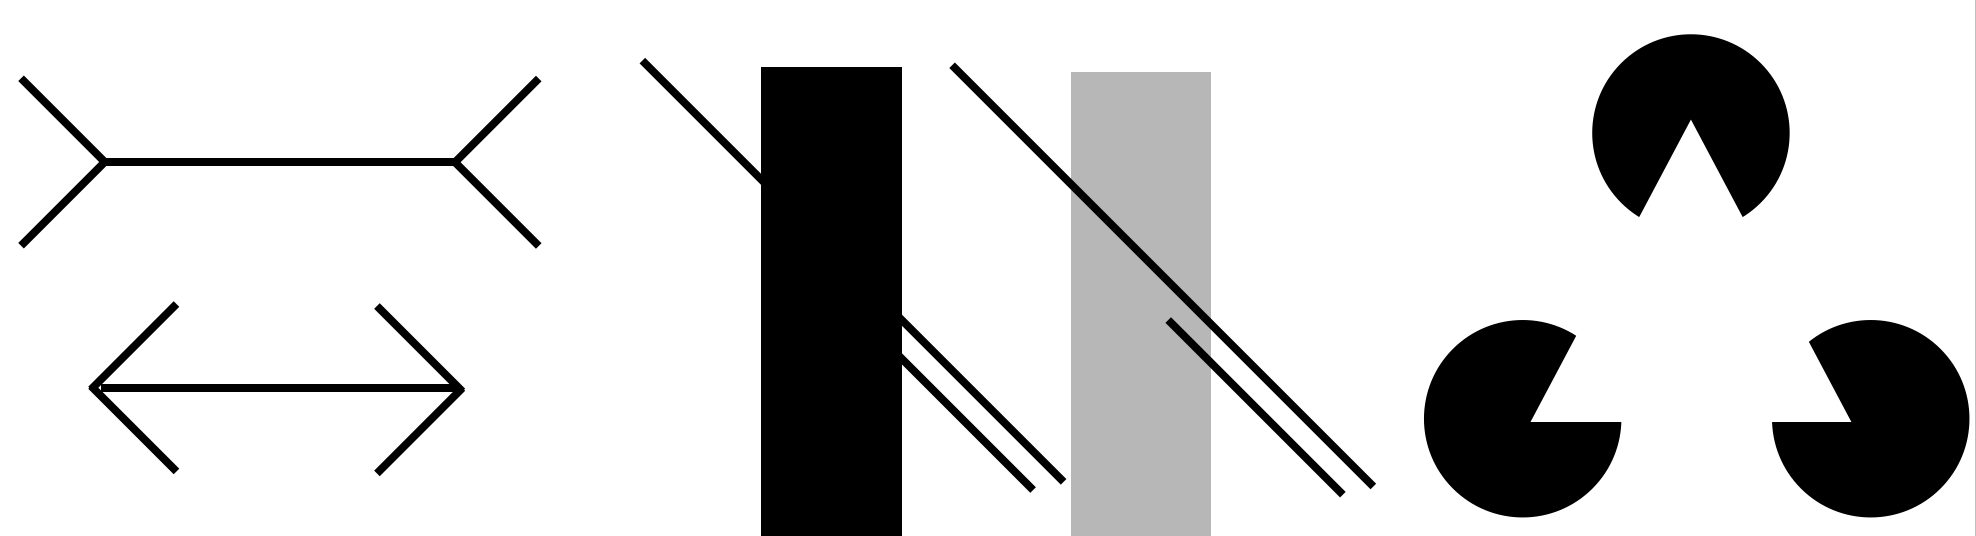
\includegraphics[keepaspectratio,width=1\linewidth]{../images/05_illusion.png}
	\caption{錯視の例。左から，ミューラー・リヤー錯視，ポッケンドルフ錯視，カニッツァの三角形}
	\label{illusions}
\end{figure}

錯聴についての話ですが，そうですね，私は中学生のとき吹奏楽部に所属していました。さらに，私には3人の子どもがいて，全員が吹奏楽部に入っています。家族の中で唯一，私の妻だけが吹奏楽や音楽の経験がないのです。なので，私や子どもたちが「この曲のベースラインがかっこいいね」とか「この曲の隅で聞こえるリフがいい感じだね」とか，「ドラムの音がどうだ」という話をするのですが，妻はそのように音の高音，中音，低音といった要素ごとに聞き分けたことがないらしく，そういった話題に加わりにくいと感じることがあるようです。

私は吹奏楽部のときチューバを担当していました。自分が演奏する低音パートやラインはしっかり把握していましたし，全体として楽曲がどのように構成されているかも，練習を積めば誰でも分かるようになると思います。ただこの音楽というのは，音符一つ一つの要素を調べただけでは，良い音や良い和音がどうしてそう感じられるのかを説明しきれないんです。たとえば，音が高いから良いとか低いからかっこいいといった単純なルールがあるわけではなく，音の間隔や組み合わせによって，「この5つの音が同時になると調和して聞こえる」とか，「真ん中の3度の音が半音下がると長調(Major)から単調(Minor)になる」など，音の配置や組み合わせが印象に大きく影響するのです。このような感覚を理解する手助けをしてくれるのが，錯視や錯聴のような現象です。興味のある方は，「イリュージョンフォーラム」というサイト\footnote{\url{https://illusion-forum.ilab.ntt.co.jp/},2024年11月3日アクセス。}がネット上にありますので，そこにアクセスしてみてください。さまざまな錯視や錯聴の例が紹介されています。

話を戻すと，ゲシュタルト心理学\index[termidx]{げしゅたるとしんりがく@ゲシュタルト心理学}は，今述べたように，音楽や視覚の要素を細かく分解しても，心というものは全体像を把握する働きを持っているので，要素に分けただけでは心の全体的な理解には至らない，という立場をとっている学派です。この学派には，シュトゥンプフ\footnote{カール・シュトゥンプフ(Carl Stumpf, 1848年4月21日 - 1936年12月25日)ドイツの哲学者・心理学者であり，音響心理学の分野で著名である。フランツ・ブレンターノやルドルフ・ロッツェのもとで学び，後にエドムント・フッサールやゲシュタルト心理学\index[termidx]{げしゅたるとしんりがく@ゲシュタルト心理学}の創始者に影響を与えた。実験心理学の先駆者として，音楽心理学と現象学的研究を重視した。(Wikipediaより)}，コフカ\footnote{クルト・コフカ(Kurt Koffka, 1886年3月18日 - 1941年11月22日)ドイツ出身の心理学者で，ゲシュタルト心理学\index[termidx]{げしゅたるとしんりがく@ゲシュタルト心理学}を体系化し，知覚心理学に貢献した。知覚や学習，記憶，発達の分野での研究が中心であり，「知覚のゲシュタルト原理」に関する理論を展開した。}，ケーラー\footnote{ヴォルフガング・ケーラー(Wolfgang K\"ohler, 1887年1月21日 - 1967年6月11日)  エストニア生まれのドイツの心理学者で，ゲシュタルト心理学\index[termidx]{げしゅたるとしんりがく@ゲシュタルト心理学}の共同創始者である。チンパンジーの洞察学習の研究で知られ，問題解決や学習の洞察に関する理論を打ち立てた。彼の研究は知覚心理学や認知心理学\index[termidx]{にんちしんりがく@認知心理学}にも大きな影響を与えた。(Wikipediaより)}，ハイダー\footnote{フリッツ・ハイダー(Fritz Heider, 1896年2月19日 - 1988年1月2日)オーストリア生まれで，アメリカで活躍した心理学者である。ゲシュタルト心理学\index[termidx]{げしゅたるとしんりがく@ゲシュタルト心理学}の影響を受け，社会的認知\index[termidx]{しゃかいてきにんち@社会的認知}や「帰属理論」および「認知的均衡理論\index[termidx]{にんちてききんこうりろん@認知的均衡理論}」を提唱した。これにより，社会心理学の発展に大きく貢献した。}，レヴィン\index[nameidx]{れゔぃん@レヴィン}\footnote{クルト・レヴィン\index[nameidx]{れゔぃん@レヴィン}(Kurt Lewin, 1890年9月9日 - 1947年2月12日) ドイツ出身の心理学者であり，後にアメリカで活動した。「場の理論」を提唱し，行動が個人と環境の相互作用により決まるとした。さらに，グループ・ダイナミクスや「アクション・リサーチ\index[termidx]{あくしょんりさーち@アクション・リサーチ}」の概念を導入し，組織心理学や社会心理学に多大な影響を与えた。(Wikipediaより)}といった有名な研究者がいます。特にハイダーやレヴィン\index[nameidx]{れゔぃん@レヴィン}は，このゲシュタルトの考え方を社会心理学の分野に取り入れました。

レヴィン\index[nameidx]{れゔぃん@レヴィン}については，後ほど詳しく触れる予定ですが，彼は『社会科学における場の理論』\parencite{Lewin}という本も執筆しています。一応，社会心理学を学んだという人は，ぜひ一度読んでいただきたい。非常に読みにくい，今風ではない文体なんですけれども，しかも何を言っているか分からないところも結構あったりするんですが，少なくとも一つ，社会心理学における場の理論という一大ムーブメントを巻き起こした考え方であります。これは何かと言いますと，FieldのTheoryなので。場(Field)というのは電磁場とか磁場とか，物理学にあるような力場のようなイメージ。心にもそういう場というのがあって，それぞれの力が相互に依存しあって影響しあって現象を作り上げるという発想です。この発想がグループダイナミクスを生んでくるスタートになりますので，この『社会科学における場の理論』，少なくともレヴィン\index[nameidx]{れゔぃん@レヴィン}の場の理論というのは，ちょっと頭の中に入れるようにしておいてください。

\section{モレノとホーソン実験}
さて，そういった話がヨーロッパの方で出てくるんですけれども，1920年代ぐらいに入りますと，社会心理学の本場がアメリカの方に移ってきます。アメリカの方にオールポート\index[nameidx]{おーるぽーと@オールポート}\footnote{ゴードン・オールポート\index[nameidx]{おーるぽーと@オールポート}(Gordon W. Allport, 1897年11月11日 - 1967年10月9日)  アメリカ合衆国の心理学者で，パーソナリティ心理学の先駆者として知られる。ハーバード大学で心理学の博士号を取得し，同大学で教鞭を執った。彼は特性論を提唱し，個人の特性を首要特性，中心特性，副次特性の三つに分類した。また，宗教心理学や偏見の研究にも貢献し，社会心理学の発展に寄与した。(Wikipediaより)}だとかマクドゥーガル\footnote{ウィリアム・マクドゥーガル(William McDougall, 1871年6月22日 - 1938年11月28日)  イギリス生まれの心理学者で，社会心理学の創始者の一人とされる。ケンブリッジ大学で医学を学び，後に心理学に転向した。1920年にアメリカへ渡り，ハーバード大学やデューク大学で教授を務めた。本能を重視し，生物学的・目的論的立場から心理学を展開した。主著に『社会心理学入門』や『集団心』がある。(Wikipediaより)}というようなアメリカの社会心理学者が出てくるというのが一つ。もう一つは「ナチスの贈り物」と言われることです。レヴィン\index[nameidx]{れゔぃん@レヴィン}とかハイダーはユダヤ人なんです。時代背景は皆さんもご存知だと思いますけれども，ナチスがユダヤ人という民族を亡くそうという活動をヨーロッパで始めますので，多くの人が亡命します。多くの人がアメリカに行きます。アメリカはどんどん受け入れたこともあって，「ナチスの贈り物」とアメリカなんかで言うらしいんですけれども，ヨーロッパの知識人がアメリカの方に亡命していきました。

亡命した人の中には，たとえばラザースフェルド\footnote{ポール・ラザースフェルド(Paul Lazarsfeld, 1901年2月13日 - 1976年8月30日)  オーストリア生まれのアメリカ合衆国の社会学者で，コロンビア大学応用社会調査研究部門の長として，定量的調査の発展をリードした。アメリカ社会学会の会長も務め，コミュニケーション\index[termidx]{こみゅにけーしょん@コミュニケーション}研究の学祖と評されている。特に，ラジオ聴取研究や『ピープルズ・チョイス』でのオピニオン・リーダーの概念提唱で知られる。(Wikipediaより)}，モレノ\index[nameidx]{もれの@モレノ}\footnote{ヤコブ・レヴィ・モレノ\index[nameidx]{もれの@モレノ}(Jacob Levy Moreno, 1889年5月18日 - 1974年5月14日)  ルーマニア生まれのオーストリア・アメリカの精神科医，心理学者，社会学者で，サイコドラマとソシオメトリーの創始者として知られる。人間関係の測定と分析を行うソシオメトリーを開発し，集団療法の分野に大きな影響を与えた。(Wikipediaより)}，アドルノ\index[nameidx]{あどるの@アドルノ}\footnote{テオドール・アドルノ\index[nameidx]{あどるの@アドルノ}(Theodor Adorno, 1903年9月11日 - 1969年8月6日)  ドイツの哲学者，社会学者，音楽学者で，フランクフルト学派の中心人物の一人。批判理論を発展させ，文化産業論や権威主義的パーソナリティの研究で知られる。ナチス政権下でアメリカに亡命し，戦後ドイツに帰国してからも多くの著作を残した。(Wikipediaより)}，フロム\footnote{エーリッヒ・フロム(Erich Fromm, 1900年3月23日 - 1980年3月18日)  ドイツ生まれのアメリカの社会心理学者，精神分析\index[termidx]{せいしんぶんせき@精神分析}学者で，フランクフルト学派に属する。人間の自由と疎外に関する研究で知られ，『自由からの逃走』や『愛するということ』などの著作を通じて，人間性の理解と社会批判を行った。(Wikipediaより)}，ハイダー，シュッツ\footnote{アルフレッド・シュッツ(Alfred Schütz, 1899年4月13日 - 1959年5月20日)  オーストリア生まれのアメリカの社会学者で，現象学的社会学の創始者。エドムント・フッサールの現象学を社会科学に応用し，日常生活の社会的構成を分析した。主著『社会的現実の意味構成』で，社会的行為の主観的意味の理解を追求した。(Wikipediaより)}，レヴィン\index[nameidx]{れゔぃん@レヴィン}という有名な人の名前があるんですが，こういった人たちがざっとアメリカに移ったことがあって，学問の基盤がアメリカの方にぐっと動くということもあるわけです。

その20年代頃にもうひとつイベントとしてアメリカの方であったのが，ワトソン\index[nameidx]{わとそん@ワトソン}の行動主義宣言ですね。あれは13年くらいにあったりしますので，そのあたりで多くの研究者がアメリカに移り，アメリカの方で社会的な科学をやりましょう。それこそ心理学といえば，ネズミを相手に実験していたという時代から，ワトソン\index[nameidx]{わとそん@ワトソン}の行動主義宣言の影響を受けて，人間を相手にそういった実験もするんだという話も始まるというのはこの頃になります。

\subsection{誰が生き残るべきか?}
ここで，2つの興味深い研究と研究者を紹介しましょう。まず，ヤコブ・レヴィ・モレノ\index[nameidx]{もれの@モレノ}という人物です。彼は臨床心理学の「サイコドラマ」という手法に大きな影響を与えており，現在もその影響は続いています。サイコドラマやソシオドラマと呼ばれるこの方法は，集団で演劇的なアプローチを通じて心理を探る手法で，モレノ\index[nameidx]{もれの@モレノ}が始めたものです。

モレノ\index[nameidx]{もれの@モレノ}という人は，\textbf{ソシオメトリー}Sociometryという社会科学を作ろうとしたんです。ソシオメトリー，日本語なら社会測定学。メトリックmetricは測定するということなので，社会を測定しましょうという学問を作ろうとしているんです。社会心理学の中には，ソシオメトリック・テストという形で導入されました。ソシオメトリック・テストというのは，モレノ\index[nameidx]{もれの@モレノ}自身がやった研究もそうなんですけど，学級集団とかで「君たち進級するにあたって，クラス替えがあったとすると，どの子と同じクラスになりたいですか？3人まであげてください」というようなことを聞くんです。もっと言うと，「好きな子3人と嫌いな子3人を言って」という感じの調査を全員にします。そういうことで，この子とこの子は仲がいいんだね，この子はこっちの友達と言うんだけど，こっちの方はそうは思ってないね，というような社会関係を全部測定しましょうという話ですね。日本の社会心理学の中に残ったのは，この人間関係を測定するソシオメトリック・テストだけなんです。ちなみに，今言った学級の中で「誰が好きですか，嫌いですか」というソシオメトリック・テストは，日本にも導入されたことがあります。学級の中でそういった調査をして，学級の中の友達関係などの調査に使われていた時期があるんです。ただ，言ったように，調査方法が，「あなたは誰が好きですか，誰が嫌いですか」ということを児童生徒に聞いて，それを名前を挙げさせるというもの。これだと，あの子が嫌いですとか，その子が言ったことによって，自分はあの子のこと嫌いなんだと明確に意識してしまうじゃないか，とか，少なくとも教育効果が教育上よくないのではないかというクレームがつきまして，日本の学校でソシオメトリック・テストをやってはいけないということになって廃れました。

ともかく，そういうソシオメトリック・テストというのは，社会心理学の中にもはいってます。「社会心理学の中には」という言い方に，ちょっと含みがあるんですけど，それは何かと言いますと，モレノ\index[nameidx]{もれの@モレノ}がやりたかったことはソシオメトリック・テストじゃないんです。ソシオメトリック・テストを今言ったような人間関係の調査法だけに限定したものは，実は本来のソシオメトリーの使い方ではないと言われています。

これは田中熊次郎という人が書いている本\footnote{「ソシオメトリーの理論と方法」，\textcite{TanakaKumajiro}です。}にもはっきり書いてあるんですけれども，そういった人間関係を調査することだけを目的にしたソシオメトリック・テストは，コールド・ソシオメトリー，冷たいソシオメトリーと言われて，本家からは嫌われるやり方なです。本来はホットなソシオメトリーをしないといけない。それは何かと言うと，測って調査して終わりじゃなくて，その人間関係や好き嫌いの関係を記録したものは，学級だったら学級の集団の状況を映し取ったカルテのようなものなんですね。カルテとって終わり，という治療がないように，このデータをもとに教師なり臨床家なり実践家の人たちが，その集団をより良くするための介入をするときの材料にしましょうというのが，本来のソシオメトリック・テストの使い方なんです。

モレノ\index[nameidx]{もれの@モレノ}がやろうとしたソシオメトリーは，ソシオメトリック・テストだけではありません。ソシオメトリック・テストは，誰が好きですか嫌いですかという情緒的な関係だけを測定しますけれども，もうちょっと単純な知人テストというのもあります。「あなた，この学級の中で知っている子は誰？」と聞く表面的なレベルの調査ですね。その他にも，たとえば教室の中に観察員や測定員のような人がいて，「誰それが，あの子と何分間会話しました」とか全部記録するというのもあります。つまり，学級の状態をこと細かく表面的な行動のレベルで全部記録するという測定の仕方だったり，役割を与えた時に，こういう時にこの子はどう振る舞うだろうかといったような，ロールプレイをさせた時の動きを見る測定方法だとか，いくつものレベルでの測定をモレノ\index[nameidx]{もれの@モレノ}は考えています。

\begin{figure}[ht]
	\centering
	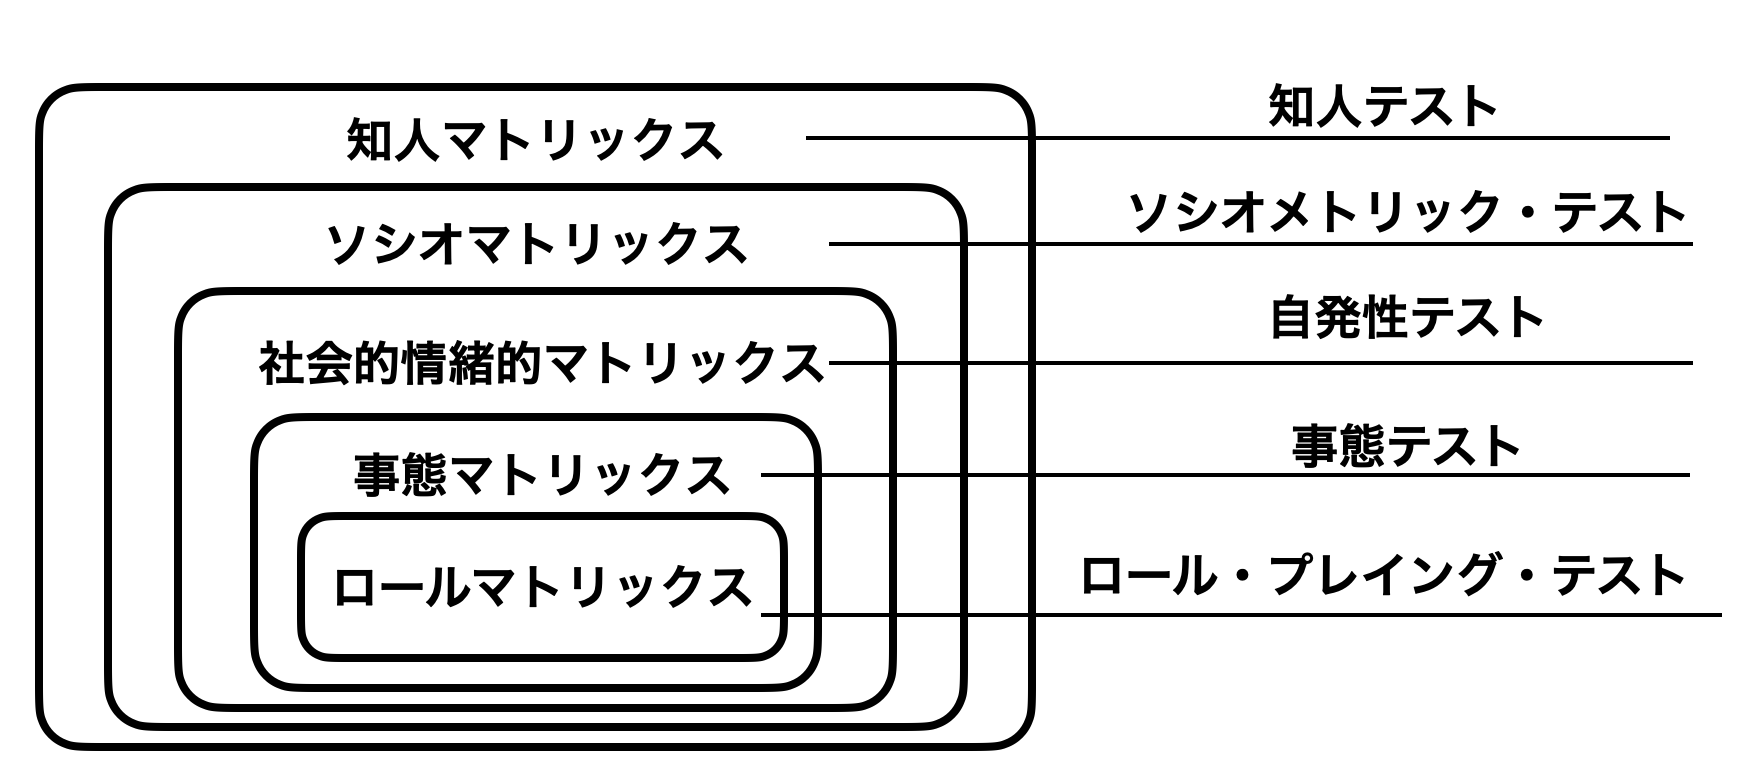
\includegraphics[keepaspectratio,width=1\linewidth]{../images/05_Sociometry.png}
	\caption{モレノ\index[nameidx]{もれの@モレノ}のソシオメトリー体型。\textcite{TanakaKumajiro}より，著者が加筆修正しました。}
	\label{illusions}
\end{figure}


それら全部を含めて社会測定学。だから別に誰と誰が仲良しかというのを調べて，そこで終わるんじゃなくて，あらゆる角度で社会集団の状態を測定して，それをデータとして，エビデンスとして，それをもとに社会を，メンバーをより活気づける方向に，働きかけをしていこう，あるいは臨床的な意味でいうと治療していこうというような動き，これがモレノ\index[nameidx]{もれの@モレノ}のやろうとしていたソシオメトリーという学問体系です。だから単なる調査手法ではないんです。社会心理学の中には，今言ったようにソシオメトリック・テストという，単なる測定法として入ってきましたけれども，本来そういうムーブメントがあったんだということは知っておいていただきたいと思います。

モレノ\index[nameidx]{もれの@モレノ}は``Who shall survive?''という本\parencite{moreno1934who}を書いています。かなり分厚い本です。私は学生の頃に指導教員に言われて読んだんですが，中身は学校の6年生から12年生ぐらいまでの，毎年ソシオメトリックな調査をしている全部の記録が載っていて，この時にどうなった，あったみたいなのを全記録だったりします。その本の最後の章で，モレノ\index[nameidx]{もれの@モレノ}が主張しているのは，``Who shall survive?''「誰が生き残るべきか?」。

当時の時代背景ももちろんあるんですが，これから先，人口がどんどん増えくだろうという時です。1920年代でどんどん増えていっているので，マルサスの人口論\footnote{トマス・ロバート・マルサス(Thomas Robert Malthus, 1766年2月13日 - 1834年12月29日)は，イギリスの経済学者・人口学者であり，1798年に『人口論』(An Essay on the Principle of Population)を著した。この著作でマルサスは，人口は幾何級数的に増加する一方，食糧などの生活資源は算術級数的にしか増加しないと主張し，人口増加が生活資源の供給を上回ることで貧困や飢餓が避けられないと論じた。また，人口増加を抑制する手段として，道徳的抑制(晩婚や禁欲)などの「予防的制限」と，戦争や疫病，飢饉などの「積極的制限」を提唱した。この理論は「マルサスの罠」として知られ，経済学や人口学に大きな影響を与えた。(Wikipediaより)}なんかも念頭にある。増えていくとそのうち人口が爆発するぞ，ということが危惧されていた。人口が爆発すると，食料危機が来ます。その時に誰が生き残るべきかということを主張している本なんです。

さて，人間にとってもっとも大事なのは何かというと，モレノ\index[nameidx]{もれの@モレノ}曰くそれは自発性spontaneouslyと創造性creativity，だそうです。そしてこの自発性と創造性をもっとも発揮している人間は何かというと，間違いなく若者，子どもだという。誰が生き残るべきか。人口爆発して，どうせ飢えて死ぬのであれば，子どもこそ生き残らせなければならない。その本には「人口の食料危機みたいなことがあったら，大体30歳を超えたら人間は死ぬべきだ。自発性と創造性がなくなっているから」という。それを読んだ時，私は20代だったので，あとちょっとかと思ったんですよ。もう今30歳は遥かに超えてしまったので，そろそろ死ななきゃいけないのかなと思うんですけど，モレノ\index[nameidx]{もれの@モレノ}はそういうメッセージを世に出しているわけです。

今も言いましたように，この人は心理学者というより実践家です。心理学の中でいうと臨床心理学的なところに，その名前が残っています。モレノ\index[nameidx]{もれの@モレノ}が実践手法としてよくやっていたのは，即興劇というやつです。急に舞台上に人を上げて，「あなたは何々の役でやってごらん」と言って，役割だけ与えて演技させるんです。セリフも何もなしでも，全部即興でやらせる。そういうのをやっていく中で，いろんな役割をそれぞれの人が演じていくことによって，人間ってこういう立場になったらこういう振る舞いをするんだなということを，客観的にも主観的にも理解させる。それをもって，そのグループをどんどん良くしていきましょうというような活動をされていた人です。

興味がある人は，モレノ\index[nameidx]{もれの@モレノ}については伝記的な本が残っていますので，よかったら読んでみてください\footnote{すみません，講義中は「エッセンシャル・モレノ\index[nameidx]{もれの@モレノ}」\parencite{essentialMoreno}とご紹介しましたが，伝記的なのは「神を演じ続けた男」\parencite{GodOfMoreno}の方でした。お詫びして訂正します。}。中には驚くような経験が書かれています。モレノ\index[nameidx]{もれの@モレノ}は自分のことを神様なんだというふうに，子供の頃は信じ込んでいた。モレノ\index[nameidx]{もれの@モレノ}が子供の頃にあった「神様と天国」という遊びがあります。これ，モレノ\index[nameidx]{もれの@モレノ}と子供達が，部屋の椅子とか机を集めて高く積み上げるんですね。で，一番上でモレノ\index[nameidx]{もれの@モレノ}がこう手をうえに挙げて，ほかの子供たちがそれを祈るという遊びらしいです。何が面白いのかわかりませんけど。こんな感じで，神様ごっことかって遊んでいたとかいう話が本に載ってます。最後は上からもレノが転げ落ちて骨折したらしいですが。あと，「自分は本当に神様に選ばれた特殊な人間なんだ」と。それを証明してみせるということで，窓から全裸で街中に飛び出した逸話とかが残ってます。なんか強烈な人だったようです。そこだけ聞くとただの変態のような気もするんですけれども，ルソー\footnote{ジャン＝ジャック・ルソー(Jean-Jacques Rousseau, 1712年6月28日 - 1778年7月2日)は，フランスの哲学者，政治哲学者，思想家である。代表的な著作に『社会契約論』や『エミール』があり，これらの作品はフランス革命や近代教育の発展に大きな影響を与えた。ルソーは人間の自由と平等を強調し，自然状態における人間の善性を主張した。また，教育においては子供の自主性と自然な成長を重視する理念を提唱した。(Wikipediaより)}も露出狂だったとかという話もあったりしますから，天才と何とかはという話なのかもしれません。

とにかくモレノ\index[nameidx]{もれの@モレノ}という人が，そういった実践活動をしてた人だということです。たとえば即興劇をやる小屋を作って，アメリカの各地で即興劇のグループワークをする。そういう活動をしたりしていたという時代があった。ということで，ちょっとこのモレノ\index[nameidx]{もれの@モレノ}という人を知っておいてください。なぜなら，モレノ\index[nameidx]{もれの@モレノ}自身はレヴィン\index[nameidx]{れゔぃん@レヴィン}のライバルだと思っていたみたいで，この後レヴィン\index[nameidx]{れゔぃん@レヴィン}の研究をちょっとご紹介するんですが，「私の研究は私の研究を剽窃したものだ」というような非難をしていたという話もあったりしますので。

\subsection{ホーソン実験}

さて，モレノ\index[nameidx]{もれの@モレノ}という人物の人柄や臨床活動はひとまず置いておいて，彼が目指した「社会測定学」。これはどうでしょうか。先ほども触れたように，モレノ\index[nameidx]{もれの@モレノ}は数十人規模の限られた集団内での人間の動きをすべて記録し，そのデータを分析して実際の活動に役立てることができると考えました。この考え方，皆さんはどう思いますか？2024年の今なら，ウェアラブルデバイスやセンサーなど，技術は100年前に比べて飛躍的に進化しています。人間の動きを記録するにしても，モレノ\index[nameidx]{もれの@モレノ}の時代よりもはるかに精密にできるはずです。機械的にミリ単位やミリ秒単位で，非常に高い精度で記録できるかもしれません。たとえば，小学生の学級内で「誰がどこに移動して，何秒間誰と関わっているか」など，すべてを細かく記録することも可能かもしれません。しかし，ここで問いかけたいのは，こうして完璧に記録を行えば，それで学級の状態や人間関係がしっかりと把握できるのか，という点です。皆さんは，この研究方針に賛成できますか？それとも，「記録しただけでは本質的な理解にはつながらない」と感じますか？

モレノ\index[nameidx]{もれの@モレノ}が取り組んでいたことは，例えば直接本人に「誰が好き？」と尋ねたり，教室の隅で調査員が「あの子と話した」などとメモを取ったりする，という活動ですよね。人のすることですから，見逃してしまったり，正確に記録できなかったりする場面も多々あったと思います。それでもモレノ\index[nameidx]{もれの@モレノ}の発想としては，「しっかりと測定し，分析をすれば，ある程度のことはわかるはずだ」というものでした。

同じような方針，考え方が垣間見える例として，「ホーソン実験」というものがあります。産業社会学などを学んだ方には，聞いたことがあるかもしれません。私も学生の頃に産業社会学の授業で，このホーソン実験について初めて詳しく学びました。ホーソン実験は，1924年から1932年にかけて，約7年間にわたって行われました。ホーソンという地名にある工場で行われた大規模な実験で，メイヨー\footnote{エルトン・メイヨー(Elton Mayo, 1880年12月26日 - 1949年9月7日)  オーストラリア出身の産業心理学者で，人間関係論の創始者として知られる。ハーバード・ビジネス・スクールで教授を務め，ウェスタン・エレクトリック社のホーソン工場で行われたホーソン実験を主導し，労働者の生産性における社会的要因の重要性を明らかにした。(Wikipediaより)}やレスリスバーガー\footnote{フリッツ・J・レスリスバーガー(Fritz J. Roethlisberger, 1898年10月29日 - 1974年5月17日)  アメリカの経営学者・組織行動研究者で，エルトン・メイヨーとともにハーバード大学でホーソン実験を指導し，非公式組織の存在やその役割を解明した。主な著書に『経営管理と労働者』や『経営と勤労意欲』がある。 (Wikipediaより)}，ホワイトヘッド\footnote{T.N.ホワイトヘッド(Tom North Whitehead, 1891年12月31日 - 1969年11月22日)  イギリス生まれの社会学者で，ハーバード大学でエルトン・メイヨーらとともにホーソン実験に参加し，労働者の社会的関係と生産性の関連性を研究した。主著に『The Industrial Worker』がある。(Wikipediaより)}といった社会科学者が多く関わっています。この実験で何をしていたかというと，工場で製品を作る際に，どのような条件や環境を整えれば生産性が向上するのかを徹底的に記録し，コントロールし，その関数関係を明らかにしようとしたのです。

社会測定学が「社会関係をすべて測定しよう」とするのと同様に，ホーソン実験でも「工場での生産性を最大化するために，どの条件が最適か」をさまざまな環境で試したわけです。そのためには，まず工場で製品を作る際の動きの最小単位をすべて書き出し，たとえば，部品を持ってきて道具を取って組み立て，隣の作業者に渡す，といった各動作を細かく分析しました。こうしたひとつひとつの作業に平均どれくらいの時間がかかるかを測定し，標準的な作業量を割り出しました。次に，「この作業量でこの給料の場合」「あるいは一定以上の生産量に達したら給料が上がる場合」など，さまざまな条件下でどの程度生産性が向上するかを調べました。ひとつあたりの単価制や出来高制，あるいはインセンティブを付けた方が良いのかといった複数の条件を試しながら，労働者のやる気を引き出す最適な方法を探し出そうとしたのです。ホーソン実験は「照明実験」から始まったんですが，これは，作業場の照明が明るいほうが良いのか，少し暗めのほうが良いのかを検証するもので，毎週異なる明るさにして生産性の変化を観察し，もっとも効率が上がる照明の強さを見つけようというものです。

何かの組み立て作業をする時も，いろんな条件，いま言ったような給料の体系とかいろいろ変えて，どうなるかというのを調べていたわけです。これが面白いことに，そうやってものすごく科学的というか，測定にこだわって合理的な工場経営をやっているわけですよね。いろんな条件を試したんですけど，ここまでの段階で分かったことは，条件を変えても，そんなにはっきりと生産性が上がる，これといった決め手というのは見つからなかったんです。大変ですねえ，結構大掛かりなことをやってたと思うんですけど，成果ゼロですよ。ただ，このホーソン実験の面白いところは，このあと作業員たちに面接を始めるところなんですよね。作業員一人一人呼んできて，「どういうつもりで働いているの？」「どんだけ頑張ろうと思ってる？」「頑張ったらこれだけ給料が上がるって言っているのに，なんで頑張らないの？」みたいなことを，一人一人にインタビューして聞いていくわけです。

こういうことをしていって，結局それを聞きながら分かったことは何かと言いますと，いま言ったような物理的な環境，たとえば工場の光の強さだとか，環境の過ごしやすさ，あるいは賃金の支払い方，どれくらい休みを入れたらいいかとかというスケジュールのコントロール，いろんな変数を実験する側は用意しているんですけど，そのどれもが決め手じゃないということ。結局何が決め手にだったかというと，人間関係なんです。休憩時間とかで労働者同士が話をするんですね。「最近また電気の明るさが変わって実験してるらしい」みたいな話をするんでしょうね，作業員たちが。そこでいろんな人たちが集まって，仲良くなる。インフォーマルな人間関係ができあがるわけです。このインフォーマルな人間関係から，情報が共有されるようになり，お互いの個性や働きぶりが認識されるようになっていくわけです。連帯感も生まれたでしょうね。そういうのを経て，インフォーマルな，つまり役職とか，外から工場経営者の方からは分からない労働者同士のつながりみたいなのが出来てきて，「あんまりやりすぎても，どうせ天井があるからあんまり作りすぎるのやめようぜ」とか，「たまにはサボらんとやってられへんな」みたいな，仲間内のルールみたいなのができちゃう。しかも，どうもそれが一番生産性に関わっているということが分かったわけです。

面白いと思いませんか? つまり，すごく機械的に合理的に，環境変数を全部コントロールすれば，このような関数で業績は上がるはずだという仮説を全部台無しにしたのは，ここで働く人間の気持ちなんです。あるいは，労働者同士の非公式的なインフォーマルなコミュニケーション\index[termidx]{こみゅにけーしょん@コミュニケーション}。表面には見えてこない，潜在的な人間関係みたいなのが，どうも一番重要ですよということが分かってきたわけです。そういう意味で，非常に示唆的なところがあると思うんですね。

私は前回前々回ぐらいから言ってますけど，20世紀初頭の頃って，たぶんですけど，ものすごく科学万歳的な，科学ってすごいというノリがあったんだと思うんです。だからこそ，工場を一つ運営しましょうというときも，全部しっかり記録して，ちゃんとやったら関数関係が見つかるはずだ，という信念がある。あるいは集団なんかも，できるだけ，今の技術も使ってできるだけ記録して，しっかりと合理的なエビデンスに基づいて計画を立てればうまくいくというような，それこそ自然科学的な，物理学的な科学観みたいなのがあるから，臨床の現場，学校の現場，工場の現場なんかで，こういうことをやろうとしているんです。

もちろん，ある程度はできている部分もあるとは思います。しかし，そこからどうしてもこぼれ落ちてしまう要素が存在します。それが，さっき述べたような「インフォーマルな」つながり，データには残らない，人間同士のつながりです。これが実は非常に大きな要素であることが見えてきたのです。

この辺が社会心理学，あるいはグループダイナミクスの原点となっているのかもしれません。もし，工学的や自然科学的なアプローチで，生産性や学級のパフォーマンスを完全に予測し，「こうすればうまくいく」といった法則がきちんと立つのであれば，それ自体が一つのサイエンスとして成り立ったかもしれません。しかし，現実にはそう簡単にいかないことがわかっています。そこで，こうした「こぼれ落ちた部分」を心理学が拾い上げようとする考え方が出てきたわけです。何だかわからないけど，人間関係とか，人と人とのつながり，完全に人を物のようにみなして，関数のピースとして扱ってもうまくいかない部分。これを科学的に捉えようとする試みが，社会心理学誕生のきっかけになったのではないかと考えられます。

皆さんはいかがお考えでしょうか。合理的に考えるとか，理屈上はそうなってますよ，こうあるべきですよという話は，どこの世界にもあることなんですけれども，ルールでこうなっているからといったところで，人間は必ずしもそのルール通りに動くわけではないんですよね。その辺をしっかり踏まえた上で，ルールを作るとか，ルールを運用するというような視点があるかどうかを考えないといけない。この視点があるかどうかを，その人間の品とか質，あるいは教養の深さというと言い過ぎでしょうか。つまり，人間をどのようなものとして見るかということについての姿勢なんです。本当に機械のピースとして見るのであれば，ルールがこうなっているんだからこの通りでしょ，ルール違反したものはアウトという，すごく杓子定規な運営の方法で社会は良くなっていくはずですが，絶対そうはならないと私は思ってます。

私が思っているだけで，本当はもっとちゃんとしたらもっとちゃんとするかもしれません。個人的には，という前提をつけていいますが，人間というのは必ず一筋縄ではいかないものだと思います。世の中完璧なことはないですし，完璧を目指すことはダメとは言いませんが，そんなに全部自然科学的，法則定立的に動くものではないというところは，人間の歴史だとかこういった研究の例なんかから，皆さんもちょっと感じ取っていただけたらいいなと思ったりもします。

\section{いんたーみっしょん；今週の読書案内}

ちょっと余談ですけれども，本の紹介として『測りすぎ』という本\parencite{muller2019hakarisugi}をご紹介しておきます。持ってきたらよかったですね。今ちょっと喋りながら思いついたので言うんですけど，『測りすぎ』という本が言わんとすることは，数値目標みたいなのを立てると必ずそれはハックされますよという点です。たとえば犯罪の検挙率をどれぐらいまで上げましょうとか，こういった目標に達するまで頑張りましょうみたいなルールを決めて，KPIでも\footnote{KPI(Key Performance Indicator)は，業績評価指標と訳され，組織やチームが目標を達成するための進捗やパフォーマンスを数値で評価する指標のこと。}何でもいいですけど，そういったルールを決めて計画立ててやることっていっぱいありますよね。そういうのは得てして，その数値目標を達成しさえすればなんでもいいみたいなことになったりして，ハックされてダメになりますよというような話がごろごろ載っている本です。数値目標は必ずハックされるというのがテーマの本なので，興味がある人は読んでみてください。

世の中にはいっぱい数値目標，計画をしっかり立ててちゃんとしないといけないという話がありますけれども，測定すると必ずそこからこぼれ落ちるものがあります。測定してもいいですけど，必ずしもそればかりではないんだということを踏まえて，それをどう捉えるかというところを考える必要があると思います。少なくとも人文社会科学的なことを考える上では，そういったアイデアってすごく大事なことだと思うんです。なので皆さんもいろいろ考えてみてください。

僕は以前，教育学部にいたのですが，そこで時々耳を疑うようなことがありました。学生にはディプロマポリシーやアドミッションポリシー，カリキュラムポリシーといった学校のミッションが示され，それをきちんと達成しなさいと指示されるのです。ある時，文科省から通知目標が示され，「教育学部なら年間何名は教員を育てなさい」というような指示があったこともありました。僕としては，授業を受けただけでその通りに成長するとは限らないし，教えたことが100\% 伝わるわけでもないと考えています。学ぶ意欲やタイミングはそれぞれ違うものですから，こうした通知目標は現実的ではないと思うわけです。

最近では「アクティブラーニング」というものが大学で流行っていますね。学生が授業をただ黙って聞いているだけではダメで，アクティブに参加しなければいけないとされています。それ自体は理解できるのですが，ある大学では「アクティブラーニングポイント」という制度を導入しました。たとえば，講義形式の授業では，座って聞くだけなのでアクティブ度が低い。反対に，英語のコミュニケーション\index[termidx]{こみゅにけーしょん@コミュニケーション}授業などで会話や演習を行う場合，アクティブ度が高いと見なされます。

さらに，教員はシラバスを書く際に，各回の授業ごとにアクティブ・ラーニングポイントをつけなさいと求められるのです。第1回の授業が講義スタイルならアクティブ度0，第2回に演習があればアクティブ度10，といった具合です。学生はその授業を受けることでアクティブ・ラーニングポイントを貯め，卒業時に「4000ポイント貯めたからアクティブだった」「2800ポイントだから彼よりアクティブではない」といった形で可視化されるのです。僕としては，大学の授業がそんな簡単なものではないと思っています。

たとえば，この授業で皆さんが静かに聞いているとしても，興味を持って集中しているならばアクティブ度は高いでしょうし，逆に興味がなければ低いでしょう。授業の形式を決めたところで，それがそのまま学生に伝わるとは限らないことは，教育者なら誰でもわかっていることです。それでも，「授業を設計しているならアクティブ度くらい点数化できるでしょ」と教育工学者は言うのです。僕は思わず授業のアクティブ度を全部0点か100点にしてやりたい気持ちになりました。

人間はゲームのキャラクターではなく，知力や素早さが数値で上がるわけではありません。僕は，人間を育てる場としての授業でこんな仕組みがあるなんておかしいと思うのですが，皆さんはいかがでしょうか。数値でスコアリングして科学的にコントロールしようとすることには，ある側面で人間の存在に対する見方が反映されています。その教育工学者の人間観には，個人的には全く賛同できません。そのスコアリングするというか，科学的にコントロールするというのは，要するにそれができるという信念の反映なんです。つまり，人間存在をどのように考えるかというところとも関わってくる話なんですよ。



話をちょっと戻しますけれども，ソシオメトリーだとか，ホーソン実験なんかの，モレノ\index[nameidx]{もれの@モレノ}の話だとか，ホーソン実験の中で分かってきたのは，人間ってそういうね，何というのかな，物みたいなピースのようにしたって無駄だよと。人間関係という，見えない，よく分からない，非科学的とは言いませんけれども，意識を持った存在ですから，物理学とはちょっと違う必要があるというようなところが，社会心理学にとって必要な発想ではないかと思います。
\section{社会心理学の成立}

本題に戻りまして，では社会心理学を始めたいと思います。1935年にマーチンソン\footnote{カール・アランモア・マーチンソン(Carl Allanmore Murchison, 1887年–1961年)は，アメリカの心理学者。心理学という分野を初期に広めた人物の一人。歴史に名を残す多くの心理学者とは異なり，マーチンソンは影響力のある理論家や研究者ではなかったが，非常に活動的な組織者，出版者，編集者として活躍した。(Wikipedia英語版より)}という人が編集した『社会心理学ハンドブック』という本\parencite{Murchinson}がアメリカで出たそうです。これが社会心理学の成立期ではないかとされています。

この1935年のハンドブックに，例のG・W・オールポート\index[nameidx]{おーるぽーと@オールポート}，第1回のときに社会心理学の定義という話をしましたが，あの定義を言ったオールポート\index[nameidx]{おーるぽーと@オールポート}による，「社会的態度\index[termidx]{しゃかいてきたいど@社会的態度}」についての章がはいっています。
これをもって社会心理学が，他の学問とはちょっと違う，独自性を持った一つの学問体系だとして成立したのではないか，と考えるんですね。いま言った社会的態度\index[termidx]{しゃかいてきたいど@社会的態度}というのは，すごく社会心理学の中の中心的な概念である，とかつて言われていたものです。これが何なのかについては，先々この授業でもしっかり触れますので，ちょっとこの35年にオールポート\index[nameidx]{おーるぽーと@オールポート}の社会的態度\index[termidx]{しゃかいてきたいど@社会的態度}というのが出てきたということを知っておいてください。

ここで社会心理学が独立しましたよ，と言いました。さて，その特徴は何かと言いますと，まずこれをもって研究の中心がヨーロッパから完全にアメリカに移った。社会心理学のメッカはアメリカだとなったのは，この頃ですね。ナチスの贈り物もあったせいがあって，中心がアメリカにきたわけです。アメリカに来たことによって，どういった学術的研究文脈の特徴があったかと言うと，一つは個人心理学です。個人のことを大事にする。アメリカというのはそういう国柄だからというのもきっとあると思うんですが，アメリカ特有の個人の意志，考え方を大事にする個人的な心理学になったということ。

もう一つは，アメリカ的なプラグマティズムです。つまり，何かわからないけれども実際に答えが出ていたら，使えたらよいという実践の学としての側面が，社会心理学の中に組み込まれるようになってきました。ちょうどこれが時代的に新行動主義の時期と重なりますね。ワトソン\index[nameidx]{わとそん@ワトソン}が言ったS-R(刺激-反応)だけではなくて，SとRの間に，オーガニズム(有機体)，あるいは認知的なロジックを考えましょうという発想です。そして，論理実証主義\index[termidx]{ろんりじっしょうしゅぎ@論理実証主義}ですね。データを取って，ロジックと照らし合わせることによって，論理の世界と実際の世界を結びつけることができるという考え方が，この社会心理学を社会心理学たらしめるように作用しました。

つまり，方法論的な個人主義であり，状況主義\index[termidx]{じょうきょうしゅぎ@状況主義}であり，論理実証主義\index[termidx]{ろんりじっしょうしゅぎ@論理実証主義}であるという，社会心理学の基本形が，この1935年に出来上がったと考えられます。1935年当時の社会心理学は，さっきも言ったように，この測定学だとかホーソン実験のように，人間関係もできるだけ科学的に扱いましょうという方向性でした。そして，さっき言ったアメリカ的なプラグマティズム的な発想，なんだか分からなくても，できたらよい，使えたらよいというところで，比較的に行動科学とか実践の科学として発展していきます。もっと言えば政策科学ですね。国が何かの教育方針なり，この後来る第二次世界大戦に向けての軍事的な方針なんかもそうなのですが，そういった何かをするときに，「人の動きというのはこうです」「こうやったらコントロールできます」というような，実践ができる人間を対象にした実践科学という立場を，どんと打ち出したのがこの時期だったのです。テキストに書いてあった言葉を引用すると，「ウルトラモダン学」。つまり超現代的な学問として，社会心理学は非常に注目されたということです。これが社会心理学が成立した時期の特徴だと言えるでしょう。

ここでの社会心理学の基本的な考え方について，その中心がヨーロッパからアメリカに移ったと言いましたが，それまでの状況を見ておく必要があります。それまでは，わりと混沌としていたというか，いろんな考え方がその中に含まれていて，社会心理学として独立する前は，人文学，社会学，統計学など，人文系の諸科学の中に心理的なことを考えるという要素が散在していました。ヨーロッパではフランス市民革命の影響もあり，全体性だとか民族的な性質のようなものを中心にした社会学的な社会心理学が中心になっていました。

社会心理学には2種類あると言われています。社会学的な社会心理学と，心理学的な社会心理学です。ヨーロッパはどちらかというと，社会学的な全体とか民族とかを中心に考える学問が主流で，アメリカに渡った研究者たちが個人主義的な，より実践的な心理学的な社会心理学を始めます。そして，この心理学的な社会心理学が，今や社会心理学の主流になっていると考えられます。今，社会心理学の多くは心理学的な社会心理学になっています。それが1935年ごろに確立したのだと理解してください。

\subsection{社会心理学の5大理論}
当時の社会心理学の中で，社会的な行動を説明する5つの大理論というものがありした。これは知識として知っておいていただきたいので，少し紹介します。社会心理学の5大理論とは，以下の通りです：
\begin{enumerate}
    \item ゲシュタルト心理学\index[termidx]{げしゅたるとしんりがく@ゲシュタルト心理学}
    \item 場の理論
    \item 学習理論
    \item 精神分析\index[termidx]{せいしんぶんせき@精神分析}
    \item 役割理論
\end{enumerate}

ゲシュタルト理論は，先ほど錯視・錯聴のところでも言ったように，人間というのは社会的な刺激を全体的に把握する，認知するという考え方です。代表的な研究者にハイダーとかアッシュ\index[nameidx]{あっしゅ@アッシュ}がいます。アッシュ\index[nameidx]{あっしゅ@アッシュ}は同調の実験をやった人ですね。ハイダーは認知均衡理論を考えた人で，バランス理論を提唱した研究者です。理論と言いながら非常にシンプルなアイデアなのですが，ハイダーのバランス理論というのは以下のような考え方です。

その人(P;Person)と人以外のもの(X)，あるいは他者(O;Other)との関係性には2種類あるとします。ユニット関係とセンチメント関係です。ユニット関係というのは，所有しているかしていないか，一単位になっているかなっていないかです。言い換えると，持っているか持っていないか。関係があるかないか，というものです。たとえば私はここにiPhoneを持っています。私とiPhoneはユニット関係にある，といえます。もう1つはセンチメント関係と言いまして，好きとか嫌いとか情緒的な要素が入っている関係です。私はA君のことが好き，B君のことが嫌いというのがセンチメント関係です。

ハイダーのバランス理論は次のように説明されます。人間はその様々な周りの認知している要素を，全体としてバランスが取れたものになるように動機づけられるという考え方です。

具体的な例を見てみましょう。ある人(P：Person)と，別の人(O：Other)，そしてある対象(X)との関係を考えます。特にユニット関係ではなく，センチメント関係だった時に，もしその人が他者のことをポジティブに捉えていて，この人があるXという対象にポジティブな態度を持っていたら，この人もそのXのことがプラスだった方がバランスが取れていることになります。

これがバランス理論の基本的なアイデアです。たとえば，私が妻のことを好きで(ポジティブ)，妻がジャイアンツファンでジャイアンツのことを好き(ポジティブ)なのに，私はジャイアンツが嫌い(ネガティブ)だとすると，これはバランスが悪い状態になります。

バランス理論では，この三者関係のプラス，マイナスの形で表現したときに，この3つの符号の積がプラスになっていればバランス状態，マイナスになっていればインバランス(アンバランス)な状態とされます。先ほどの例では，プラス，プラス，マイナスとなり，掛け合わせるとマイナスになるので，インバランスな関係ということになります(図 \ref{balance})。

\begin{figure}[ht]
	\centering
	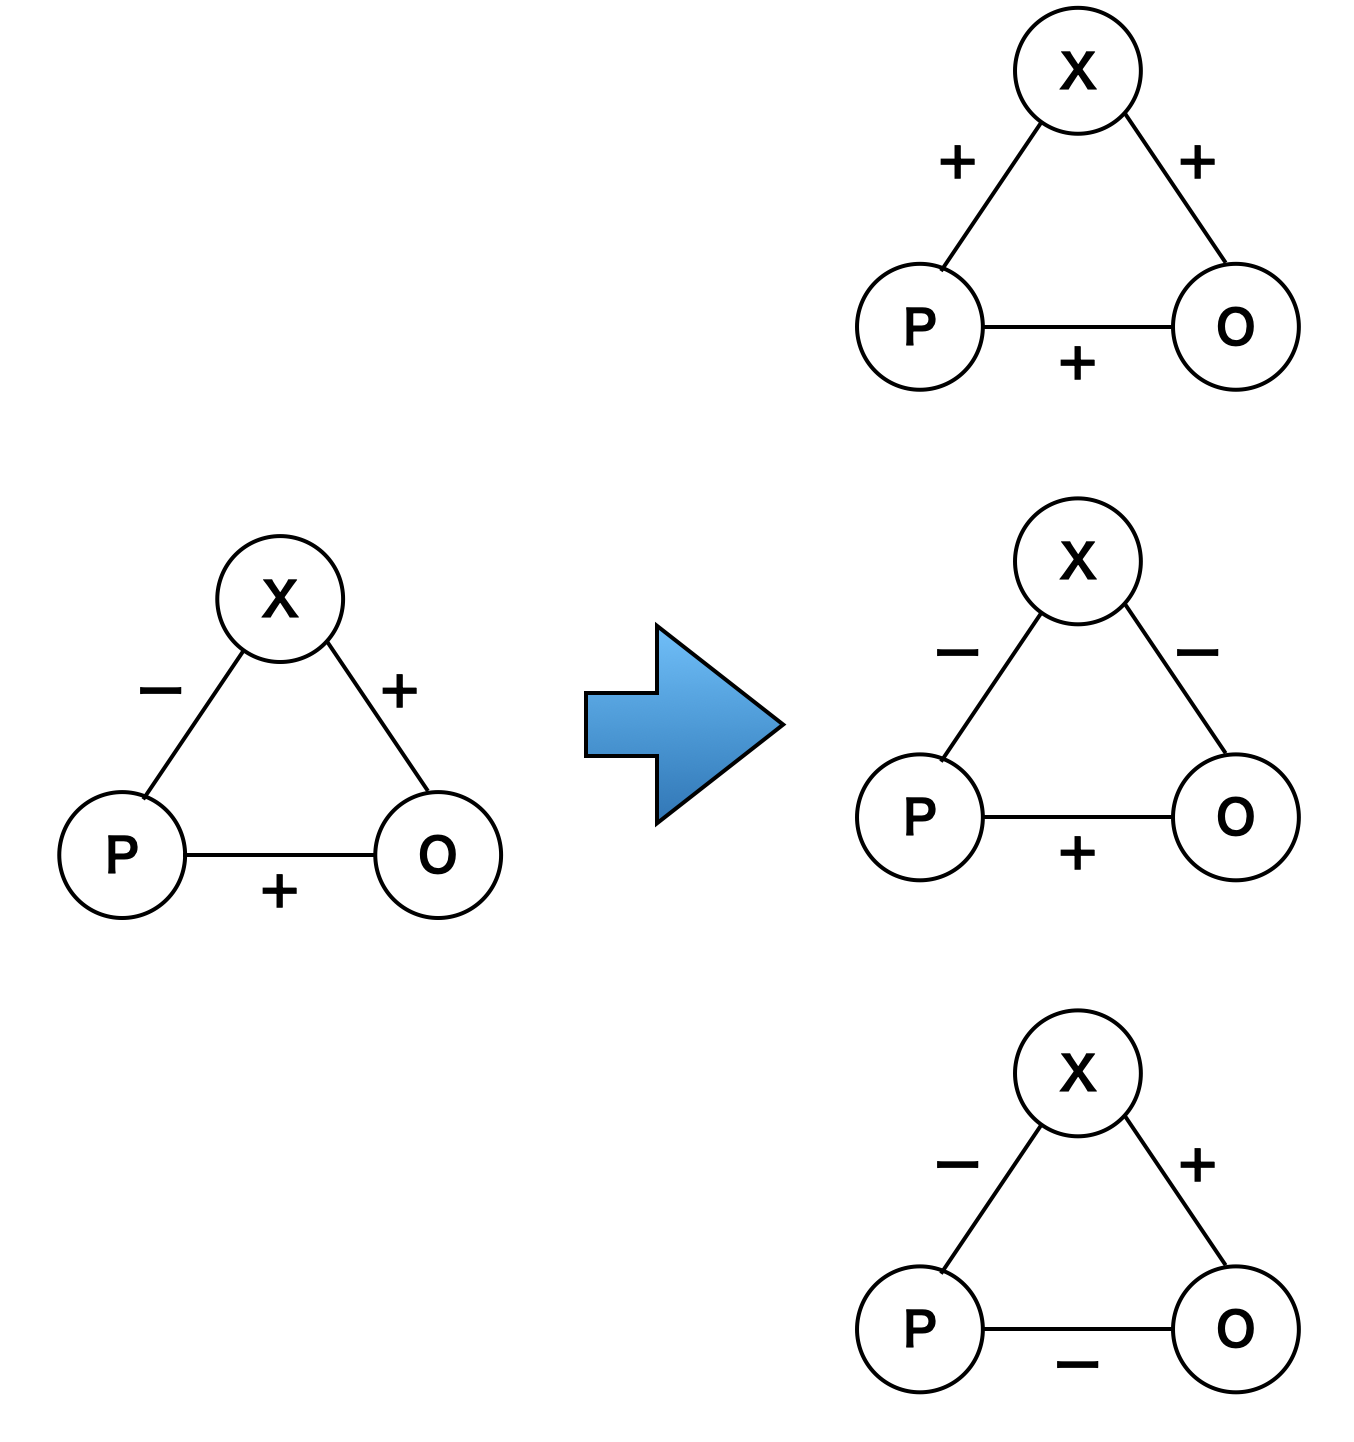
\includegraphics[keepaspectratio,width=0.5\linewidth]{../images/05_inbalance.png}
	\caption{バランス理論(POX理論)}
	\label{balance}
\end{figure}

このインバランスな状態を解消するために，人はどのように動機づけられるのでしょうか。先ほどの例で言えば，次の3つの方法が考えられます：
\begin{itemize}
    \item 自分もジャイアンツのことが好きになる
    \item 妻はジャイアンツのことを言っているけれども，本当は好きではないのだと思い込む
    \item 妻のことを嫌いになる
\end{itemize}

こんなふうにインバランスな状態であれはバランスのとれた状態に，考え方を変える，あるいは行動を変えるというのがハイダーのバランス理論です。この三者関係，三項関係のプラス，マイナスの符号の積がプラスになっていればバランス，マイナスになっていればインバランスと考えます。

ゲシュタルト的と言われるのは，この三者関係，三項関係を一体として，全体として人は捉えているという点です。一つ一つの関係で見ているのではなくて，全体を見て，今バランスしているかインバランスなのかという状態を把握します。そういうスタイルの説明の仕方をする，これがゲシュタルト理論的な社会関係の説明方法だというわけです。

この理論の提唱者，フリッツ・ハイダーという人の書いている『ある心理学者の生涯』という自叙伝\parencite{HeiderDiary}も面白いですよ。その自叙伝を見ると，バランス理論を思いついた経緯が説明されています。すごく不思議な文体で書かれていまして，ハイダーがあるお茶会に呼ばれた時に，ある男性が妻の目の前で別の女性に色目を使って，何かをしたときに妻が不快な様子を示した。そのシーンを見ていた時にハイダー自身がふわっと，「そういう関係なのだ」ということが分かったと書いてあります。その本，つまり自叙伝なのですが，全体的にずっと何が言いたいのだろうというような，ふわふわしたことが続く本なので，面白いものです。よかったら読んでみてください。その人間関係，人間が見える社会的なものの関係の把握の仕方，心の安寧の取り方のようなことを，ハイダーは考えていたようです。ハイダーもレヴィン\index[nameidx]{れゔぃん@レヴィン}と非常に親密な関係にあったので，これも場の理論とは言いませんけれども，ゲシュタルト的な意味では，ゲシュタルト学派ですし，レヴィン\index[nameidx]{れゔぃん@レヴィン}もゲシュタルトの研究者だったので，同じような発想だと考えられます。

その次に，レヴィン\index[nameidx]{れゔぃん@レヴィン}やフェスティンガー\index[nameidx]{ふぇすてぃんがー@フェスティンガー}という名前が有名な研究者がでてくる，\textbf{場の理論}があります。場の理論というのは，もう少しグループに限定した話になります。ハイダーらの話は，なんとなく人間関係というぐらいの話なのですが，レヴィン\index[nameidx]{れゔぃん@レヴィン}ははっきりとグループのダイナミクスだという話をします。

そのグループのダイナミクスが起こる力の及ぶ範囲を，レヴィン\index[nameidx]{れゔぃん@レヴィン}は場(フィールド)，心理学的なフィールドと説明します。これはゲシュタルト理論の中の1つ，特に発展した立場として挙げられます。

3つ目に挙げました学習理論というのは，強化理論とも言います。別名でよく知られているのは，条件づけですね。行動主義的な発想です。つまり，褒められた行動とか良かった行動，メリットがあった行動というのは，その出現回数が増えます。一方，やって失敗した行動，損をした行動，ネガティブな結果になったものについては，その発生回数が減りますという学習理論に基づいて，人間の社会行動を説明しようとするものです。

4つ目の精神分析\index[termidx]{せいしんぶんせき@精神分析}というのは，フロイトやユング\index[nameidx]{ゆんぐ@ユング}\footnote{カール・グスタフ・ユング\index[nameidx]{ゆんぐ@ユング}(Carl Gustav Jung，1875年7月26日-1961年6月6日)は，スイスの精神科医・心理学者であり，分析心理学(ユング\index[nameidx]{ゆんぐ@ユング}心理学)の創始者として知られる。(Wikipediaより)}，エリクソン\footnote{エリク・ホーンブルガー・エリクソン(Erik Homburger Erikson, 1902年6月15日 - 1994年5月12日)は，アメリカ合衆国の発達心理学者であり，精神分析\index[termidx]{せいしんぶんせき@精神分析}家。彼は「アイデンティティ」の概念や，心理社会的発達理論を提唱し，米国で最も影響力のあった精神分析\index[termidx]{せいしんぶんせき@精神分析}家の一人とされている。(Wikipediaより)}，フロム\footnote{エーリッヒ・フロム(Erich Fromm，1900年3月23日 - 1980年3月18日)は，ドイツ生まれのユダヤ系社会心理学者，精神分析\index[termidx]{せいしんぶんせき@精神分析}家，哲学者。フロイトの精神分析\index[termidx]{せいしんぶんせき@精神分析}とマルクス主義を融合させ，社会的性格論を提唱。代表作に『自由からの逃走』があり，ファシズムの心理的起源を分析した。(Wikipediaより)}らの理論です。これは前回お話しした内容ですね。人間が精神活動を行っているのは，ただの物理的なエネルギーだけではなくて，精神活動のエネルギーというものがあるはずだという考え方です。このエネルギーを「リビドー」や「エス(es)」，生きるためのエネルギーのような，精神のエネルギー源のようなものが腹の底から湧き出ていて，社会性とぶつかったところで人間の行動なりエゴなりが生成されるという考え方です。これによって社会行動を説明しようとする立場です。

最後の役割理論というのは，ジョージ・ハーバート・ミードの象徴的相互作用論(シンボリック・インタラクショニズム)という考え方があります。何かというと，頭の中で社会関係とかを相互に操作し合って，人は社会関係を営んでいるという考え方です。そういう意味では，たとえば私は今教師という役割を演じているし，皆さんは今学生という役割を演じています。なぜならそれがこういう場だと相互に認識しているからです。このような役割的な側面によって人間の社会行動を説明しようとする学派だというわけです。

これらが当時の社会心理学ハンドブックの中にあった5つの大きな説明原理だと言われています。その中でも説明が後々になっておりましたが，いよいよレヴィン\index[nameidx]{れゔぃん@レヴィン}のグループダイナミクスについてご説明をしていきたいと思います。

\section{レヴィンのグループ・ダイナミックス}

クルト・レヴィン\index[nameidx]{れゔぃん@レヴィン}という人なのですが，『社会科学における場の理論』という著作\parencite{Lewin}が有名だという話をしました。もう一つ，この人はものすごくたくさんの弟子を育てています。非常に研究熱心な方だったようで，大学の中だけでなく，喫茶店なんかでも，議論に参加しに来た人とは常に活発なやり取りをして，人間関係，社会関係をどうやって表現・分析するかということを考え続けていた人です。弟子の中にはフェスティンガー\index[nameidx]{ふぇすてぃんがー@フェスティンガー}，シャクター\footnote{スタンレー・シャクター(Stanley Schachter, 1922年4月15日 - 1997年6月7日)は，アメリカの心理学者で，情動の二要因理論の提唱者として知られる。(Wikipediaより)}，カートライト\footnote{ドーウィン・フィリップ・カートライト(Dorwin Philip Cartwright, 1915年3月3日 – 2008年7月18日)は，アメリカの社会心理学者で，グループダイナミクス分野の創始者の一人。彼の研究と著作は，グループダイナミクスの数学的基盤，社会的権力の源泉，グループ構造の性質，グループにおけるリスクテイクの原因などをテーマとしている。(英語版Wikipediaより)}，ドイッチ\footnote{モートン・ドイッチ(Morton Deutsch, 1920年2月4日 – 2017年3月13日)は，アメリカの社会心理学者，精神分析\index[termidx]{せいしんぶんせき@精神分析}家であり，紛争解決の研究者。(英語版Wikipediaより)}，アッシュ\index[nameidx]{あっしゅ@アッシュ}，ケリーが含まれるという話です。いま挙げた人の名前は全く覚える必要はありません。本を読んだときに出てきたら，「そうですか，有名な方ですね」と思っていただくぐらいでいいかと思います。ちなみに，ケリーという人はレヴィン\index[nameidx]{れゔぃん@レヴィン}の最後の弟子です。このケリーは，私の恩師が会ったことがあると言っていましたから，それぐらいの距離感の人です。ケリーの相互依存性理論などは結構有名なのですが，ともかくレヴィン\index[nameidx]{れゔぃん@レヴィン}は多くの弟子を育てた教育者でもある研究者だったわけです。

このレヴィン\index[nameidx]{れゔぃん@レヴィン}という人がグループダイナミクスの父といわれます。彼の基本的なアイデアは，次の式で表現されます。

$$B = f(P,E)$$

これは何かというと，Behaviour(行動)は，Personality(パーソナリティ)とEnvironment(環境)の関数ですという考え方です。数学が得意な人にとっては，何の要素を指しているのか，この関数形は何なのか，これは微分可能なのかどうかとか，いろんな批判点があるかと思います。しかし，まずご理解いただきたいのは，時代的な背景として，人間を実践的な研究対象にするということが，まだまだ画期的な時代だったので，人の行動というのは何らかの関数の形で表現できるに違いないと言っただけでも，すごいことだったということです。

この関数形がどういうものかは全然分かっていないのです。しかもレヴィン\index[nameidx]{れゔぃん@レヴィン}は，「人格というのは環境の関数($P=f(E)$)だし，環境というのはパーソナリティの関数($E=f(P)$)だ」とも言ってます。多分それぞれの関数系は全然別なんですけど，ともかくこのようなことを言うので，何が何なのかというのが気になってしかたないです。でも，少なくともこういった数学的な，あるいは力学的な関係を考えようとしたということは評価すべきだと思います。


レヴィン\index[nameidx]{れゔぃん@レヴィン}が考えていたのは次のようなことです。今から考えようとするような，例えばこの教室の中のことを考えようとしたとします。この場のことを考えますというのは，こういう生活空間(Life Space)の中に，みんなのそれぞれの人の要素があるということです。例えば，ここに小杉の要素がある，ここに学生さんA，B，Cなど，いろんな人の要素があります。これだけではありません。このときに，何か我々の行動なり考え方なりに影響を及ぼし得る認知的な要素があれば，それもこの中に書き込みます。以前に話した社会的な実在，小さな妖精さんのような要素ですとか，そういったものがあれば，それも全部書き込みます。それはみんながどういう成育歴を持っているかとか，心身の状態とか，そのほか無数の影響源があって，詳細は分からないけれども，まずある瞬間，この要素があると考えて，これが次の時点，$t$が$t+1$の時点になったときに，この変化量だけを考えよ，というのです。変化量だけを考えるのであれば，皆さんがここの部屋に入ってくるまで，どんな人生を送ってきたかとか，どんな要素があるかとかは考えなくてもよいです。

今この瞬間にある，考えるべき心理学的な要素を列挙することができれば，それが時間とともにどう変化するかということを，この認知的な空間のトポロジー空間(位相空間\index[termidx]{いそうくうかん@位相空間}という言い方もするのですが)，こういうものがあるとしたら，その空間の中での変化量は研究できる，あるいはこんな感じで関数として表現できるというのです。もちろん，たとえば私が今考えていることとか，皆さんが今頭の中に持っていることとか，ここにいるかもしれない小さな妖精さんがどれだけ入っているのかといったことが，全部測定できているわけではありません。しかし，いずれできたとして，あるいは全部書き込めたとすると，その時点とその次の$t+1$時点の変化量についてのダイナミクスを，サイエンスすることができる!という考え方を打ち出したのです。

当時の数学の発展の程度の問題，測定技術の問題もあったし，何を測定するかという問題についてもまだまだ不完全で説明も不十分だったのですが，少なくともそういう研究の方向性を示したということが偉大だったのだと理解していただけると嬉しいと思います。

このトポロジー的に描かれる生活空間，この鱗状の表現もまた，重要なポイントです。なぜかというと，全部この空間の中にそれぞれの要素が入っていて，たとえば私がとあるアクションをしたとします。私がある学生さんに「そこで何をしているのか！」と授業中に言ったとする。そうすると言われた人はびっくりして，「すみません」とか「こうしていました」と反応する，そういった変化が出るでしょう。

それは当然なのですが，このトポロジー的に描いてあるところの重要な点は何かというと，この人が行ったアクションというのは，他のところにも全部伝播していくということです。つまり，1箇所の動きがその他の要素，たとえば，一番前に座っていた学生さんが居眠りをしていたことを私が強く注意したら，その学生は確かに目を覚ますかもしれないけれど，それだけでなく「あの人が注意されたから私も気をつけよう」というように，他の人にもその影響は伝播していくのです(図 \ref{field})。

\begin{figure}[ht]
	\centering
	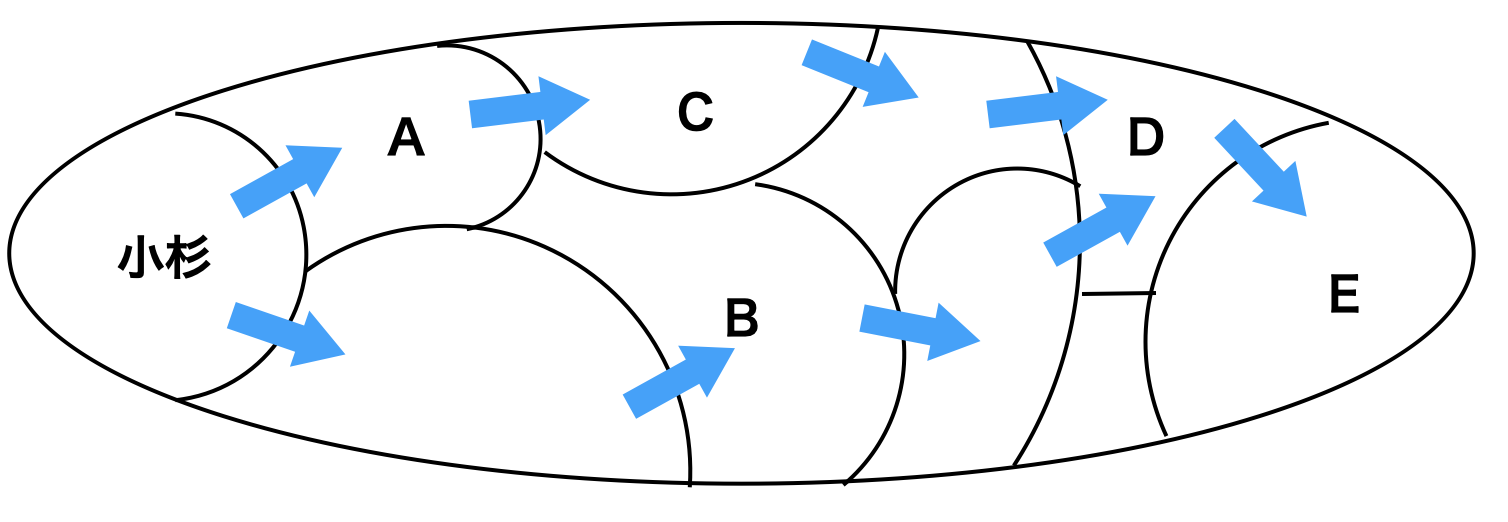
\includegraphics[keepaspectratio,width=0.7\linewidth]{../images/05_fieldtheory.png}
	\caption{場の理論における生活空間のイメージ}
	\label{field}
\end{figure}

そういった形で，このフィールドにおける一つのアクションは決して1対1の関係ではなくて，すべてが連鎖的につながっているということが，この生活空間Life Spaceの考え方です。しかも先ほど言ったように，一人一人の人間の，この教室で今から考えないといけないこのフィールド以外のところは一旦捨ておいてよい。このフィールドの中での力関係の変化量を，社会心理学やグループダイナミクスの研究対象にするのだという考え方です。これがレヴィン\index[nameidx]{れゔぃん@レヴィン}の基本的なエッセンスです。この場において，この力の及ぶ範囲として区切られるライフスペースをしっかり測定して考えることができれば，集団がどのように変わっていくかを理解することができる。このフィールドというか，ライフスペースという全体性の発想が，ゲシュタルト心理学\index[termidx]{げしゅたるとしんりがく@ゲシュタルト心理学}の影響を受けているわけです。

これのダイナミクス，変化量を考えるのだと言い切ったこと，しかもこれが一部の切り取られた世界観なので，このダイナミックな全体性がグループなのだということを言ったことをもって，レヴィン\index[nameidx]{れゔぃん@レヴィン}は「グループダイナミクス」と名付けました。グループサイコロジーではなくて，\textbf{グループダイナミクス}なのです。彼がやりたかったことは力学だったのです。もちろん完全にはできていません。なぜなら何を変数として測定しているか，関数形はどうなのかということについては，詳細をなにひとつ書ききっていないからです。ただ，おそらく彼はそれがいずれできるという考えはあったようです。すくなくとも，そちらの方向を目指してはいました。20世紀初頭の科学万歳の時代に，人間関係や社会関係というものを考える学問，力学が作れるはずだというビジョンを持って動いていた，このことの斬新さを感じ取っていただければと思います。

レヴィン\index[nameidx]{れゔぃん@レヴィン}が重視するのは相互依存性(inter-dependency)です。相互に依存するこのフィールドの要素を使ったA Dynamic Whole，つまり力動的な全体性のことを学問にするのだということで，グループダイナミクスを構築していきます。

レヴィン\index[nameidx]{れゔぃん@レヴィン}の研究として有名なものがいくつかあります。一つはリーダーシップの研究です。学校の先生のような立場の人を3つのタイプのリーダーとして用意します。
\begin{itemize}
    \item 専制君主的なリーダー：「お前はこの作業をしなさい，おしゃべりは禁止」という厳しい先生
    \item 自由放任主義の先生：「好きにしなさい，自学自習で」という感じの先生
    \item 民主的な先生：「みんな今日はどんな勉強をしようか，こうやってみようか，よし，じゃあみんなで決めてやってみよう」という感じの先生
\end{itemize}

このように全然種類の違うリーダーがいて，教えられる児童生徒たちは3人の先生それぞれの授業を受けていきます。さあ，どのリーダーシップの先生が一番パフォーマンスを上げたでしょうか。当然のことながら，民主的な先生のやり方が一番よかったという結果が出ました。

この研究の他にも，戦時下における興味深い実験があります。戦争というのはものすごくお金とか物資がかかりますから，大事なものは戦場に送って，市民たちは普段食べ慣れていない，あるいは人工的な食べ物を食べざるを得ない状況になります。しかし，みんな普段食べ慣れていないから「こんなもの食べるのは嫌だ」と思っている。では，そういった意識はどうやったら変わるかという実験をしました。全員でディスカッションをしたり，いろいろ試行錯誤して，みんなで「これを食べましょう」と決めたら，みんなが食べるようになったという集団食習慣の変容実験です。

こうやったらこのグループの中でのダイナミクスによって，人の動きや態度は変わりますよと。先ほどの学校の先生のリーダーシップの話でいえば，同じ児童生徒でやったとしても，状況が変わるだけでこんなにパフォーマンスが変わるでしょうという話をするわけです。このように，すごく実践的な人間を相手にした研究例を積み上げながら，「みんなが自分で決めていくと，集団は変わっていくのだ」「ダイナミックに全体は変わっていくのだ」ということを実証してみせているわけです。

今の話からも皆さんお分かりのように，ちょうど第二次世界大戦が近づいてきておりましたから，軍隊におけるパフォーマンス，何をもってパフォーマンスというかは考えどころですが，軍はいくつかの小隊などに分かれていますから，それぞれのグループのパフォーマンスを上げるためにはどういうリーダーシップがいいかという話は，より実践的にすごく重要だったわけです。レヴィン\index[nameidx]{れゔぃん@レヴィン}の研究のやり方のテーゼの一つに「良い理論ほど実践的なものはない」という言い方があります。つまり，どうなるかわからないアイデアがあるにしても，こういう時にこうしたらどうなるかということは，やはり現場現場で実践して，役に立つ理論でないと意味がないのだ，というようなことです。

この研究スタイルのことを「\textbf{アクション・リサーチ\index[termidx]{あくしょんりさーち@アクション・リサーチ}}」と呼びます。グループダイナミクスの研究というのは，一つには先ほどのようなトポロジー的な図を書いたりする，理論的な話もするのですが，これがいかに実践的なものを説明できるか，いかに操作可能な変数，リサーチ・クエスチョンに落とせるかということが重要なのだと力説した人でもあります。
実践だけしていてはいけない。理論だけしていてもいけない。ちゃんと使える理論を考えるのだ。このような考えで，レヴィン\index[nameidx]{れゔぃん@レヴィン}は精力的にあちこちでこういう活動をして，グループダイナミクスという学問を作り上げていったわけです。

レヴィン\index[nameidx]{れゔぃん@レヴィン}は，マサチューセッツ工科大学(MIT)にグループダイナミクス研究センターを作ります。今はミシガン大学に移設されているという話なのですが，グループダイナミクス研究センターを作って，多くの弟子を育て，このグループの力というものを研究していこうとしました。研究所を作ったりするというパワフルな人でもあったのです。

同時に，先ほども言いましたが，この人はユダヤ人でした。シオニズム運動，つまりユダヤ人救済運動(これはパレスティナ問題にも直結する話です)，ユダヤ人のための国家が必要だという運動にも非常に積極的で，研究もしながら，そういう社会運動もしながら，ものすごく一生懸命働いたせいで，割と若いうちに心臓発作でなくなってしまいます。このように超天才的な人物で，場の理論やここまでお話しした考え方は残っているのですが，その後，場の理論に基づく他の研究者やグループダイナミクスという学問がどうなったかというと，彼ほどのインパクトがある人は出てこなかったのかなという気もします。

\section{そのほかの諸研究}

ここまで，社会心理学のごく初期に，一つは個人主義的な社会心理学というのがあって，もう一つは社会心理学から一つ，独立した形でグループダイナミクスという学問ができたのが，この時期だということをお話ししてきました。

あと，ちょっとだけ補足をしておきます。先ほど私が，オールポート\index[nameidx]{おーるぽーと@オールポート}の社会的態度\index[termidx]{しゃかいてきたいど@社会的態度}というのが後々効いてきますよという話もしましたが，もう一つ大事な話があります。それは何かというと，ラザースフェルドという人が調査法を確立したという話です。

1936年の大統領選挙の予測で，リテラリー・ダイジェストという会社が，事前予測したのが大幅に外れます。これで，何人かの聞き取り調査のようなものを研究していたのですが，それではうまくいかないということで，これからはランダムサンプリング，無作為抽出法によって，均等に意見を取っていけば，もっと正確に選挙予測ができるはずだということで，社会調査の方法が確立してくるのが，この1930年代後半なのです。

なぜ私はここをそんなに強調するかというと，社会心理学の研究法として，実験・観察・調査という方法があるという話をしましたが，その調査法のスタートがこの辺なのです。この調査法で，政治学者が何を測っているかというと，政治的な態度だからよいのですが，社会心理学者はもっと一般的に社会的な態度というのを測定するのだ，そういう研究があるのだという話をするわけです。それのスタートがこの1935年あたりにあるわけです。このような社会的態度\index[termidx]{しゃかいてきたいど@社会的態度}の話と，調査法という方法論の確立は，今の社会心理学の現状に直結するような勢いで影響を与えていますから，ここは一応触れておこうと思いました。

さらに，先ほど言いましたハイダーのバランス理論は，実はハイダーの話にとどまらず広がっていきます。ハイダーが考えたこのバランス理論は，あくまでも個人の社会的刺激に対する認知の話なのです。つまり，個人の頭の中で私が社会関係をどのように捉えるか，その捉え方はインバランスなものよりもバランスの方が望ましいというふうに捉える。これがハイダーの考え方だったのです。

さらに同じような考え方をいろんな人がでてきます。
先に言ってしまいましたが，私がP(Person)とO(Other)とX(対象)で書いてありましたけれども，ハイダーはPOX理論とも呼ばれます。続いて出てきた，ニューカム\index[nameidx]{にゅーかむ@ニューカム}という人が考えたのがABX理論というものです。これは何かというと，AさんとBさんが対象Xについて話している。このAさんもBさんも人です。こういうやりとりがあるという話ですね。このAさん，Bさん，対象Xの中でのバランス関係の話をするのがニューカム\index[nameidx]{にゅーかむ@ニューカム}のバランス理論です。ニューカム\index[nameidx]{にゅーかむ@ニューカム}も認知的なバランスのようなことを考えているのですが，先ほど言ったように「私は妻が好き，私はジャイアンツが嫌い，妻はジャイアンツが好き」というので，バランス関係がうまくいかなくなると，この2人の間でコミュニケーション\index[termidx]{こみゅにけーしょん@コミュニケーション}が生じますよというような，対人認知の話というよりはコミュニケーション\index[termidx]{こみゅにけーしょん@コミュニケーション}関係の話に焦点を当てるという意味で，同じバランス的な構造の説明はするのですが，ちょっと違いがあります。もう一つ，PSC理論というのがあります。ある人が，とある内容について，どこからニュースを持ってきたかということを考えます。これも，たとえば白衣を着た賢そうな人が「この薬は効果がありますよ」というときと，街中の酔っぱらいのおじさんような人が「この薬は効果がありますよ」というときでは，絶対前者の方が印象がいいですよね。これ，その人がニュースソースとそのコンテンツの間で，整合性が取れているかどうかによって納得の程度が違うという話です。これがPSC理論。オズグッドとタネンバウム\index[nameidx]{たねんばうむ@タネンバウム}という人が考えているモデルなのですが，そういうコミュニケーション\index[termidx]{こみゅにけーしょん@コミュニケーション}におけるバランス関係を考えています。

基本的には，掛け算してプラスになったらOKというバランス理論という意味で，同じというか似ているのですが，このような研究を全部まとめて，\textbf{認知的均衡理論\index[termidx]{にんちてききんこうりろん@認知的均衡理論}}と呼んだりします。要は全部同じように認知的なレベルでの均衡，バランスが取れているかどうかを題材にしている研究だということで，これらの研究をまとめてこのように呼ぶことがあります。なぜ私がここだけ詳しく説明するかというと，先ほどハイダーの話がスタートになって，その後こういうのが出てきているのですが，おそらく社会心理学における「理論」という，でっかい理論といったのは，このバランス理論か，認知的均衡理論\index[termidx]{にんちてききんこうりろん@認知的均衡理論}群ぐらいなのではないかと思うからです。ちなみにこの認知的均衡理論\index[termidx]{にんちてききんこうりろん@認知的均衡理論}という括り方をすると，フェスティンガー\index[nameidx]{ふぇすてぃんがー@フェスティンガー}の認知的不協和の理論も含まれます。フェスティンガー\index[nameidx]{ふぇすてぃんがー@フェスティンガー}の認知的不協和の理論というのも，不協和が起きないように自分の考え方なり行動なりを変えましょうという話です。そういう意味では，バランスが取れていないよりは取れている方向に自分の心の持ちようを変えますよという意味で同じです。

これらの研究のウィークポイントは何かというと，とくに認知的不協和の理論で言われるのは次のようなことです。バランスを取りますよと言ったときの，この要素とこの要素とこの要素。3つの要素はA,B,CでもP,O,Xでもいいんです。認知的不協和の理論は認知要素ならなんでもいい。何か3つの要素を立てて，その中のバランスが取れているかどうかという話をするのですが，その認知的な要素の単位というのは明確にしないのです。「これとこれとこれのバランスの中でこいつは行動を変えたのだろう」というような説明の仕方をするので，この理論というのはどんな現象にでも当てはまってしまいます。ことわざにも「理屈と膏薬はどこにでもつく」といいますが，「きっとこいつはここでバランスを取ったのだろう」というような言い方をしたら，なんとでも筋が通った話ができてしまうのです。そういった「ちょっとオールマイティすぎる理論」という意味で，これらの認知的均衡理論\index[termidx]{にんちてききんこうりろん@認知的均衡理論}群は批判されるのですが，人の行動や態度を説明するときなどにはすごく使いやすい理論なので，よく知られています。

\vspace{2cm}

はい，今日は時間内にちゃんと社会心理学を成立させることができました。よかった。1935年から50年ぐらいの間にこういったいろんな社会心理学の芽があったのが，花開いていくつかの理論のようなものが出てきて，少なくともアメリカにおける社会心理学というのはこういう道で行くのだというのが，はっきりしたのがこの時代にあったのだということです。1935年ですから第二次世界大戦が近いですね。大戦後は日本にもグループダイナミクスだとか社会心理学は導入されます。もちろんそれ以前にも日本で研究者はいたのですけれど，本格的に導入されるのは戦後ですね。そういうことで日本でも社会心理学会，グループダイナミクス学会ができました。日本のグループダイナミクス学会は社会心理学会の歴史が古いです。より実践的な方から入ってきた，ということでしょうか。ともかく日本にも，社会心理学はこの後どんどん発展していきます。一応，社会科学としていろんな社会関係や人間関係の説明体系を作ろうとしています。「何にでも当てはまるのでは」とか「要素が分からない」「関数形が分からない」みたいな問題がいっぱいあるのですけど，こういう方向性を目指すものとして社会心理学ができあがりましたというところで，今日の話はとどめておきたいと思います。


次回はこの社会心理学が1970年代に入って混乱期，混沌期を迎えて，2000年を超えて社会心理学の危機が訪れるというところまでお話しして，この歴史シリーズを終わりにしたいと思います。
今日の話もまた講義録をまとめますけれども，もしよかったらLMSの方でコメントをいただけましたら幸いです。では今日の話はここまでにしておきましょう。

\printbibliography[title=引用文献]

\end{document}

